\documentclass[11pt,a4paper]{article}
\usepackage{amsmath,amssymb,amsfonts}
\usepackage{graphicx}
\usepackage{xcolor}
\usepackage[hidelinks]{hyperref}
\usepackage{microtype}
\usepackage{booktabs}

\begin{document}

\title{TAKT: A Formal Framework for Minimal Decision-Preserving Runtime Governance}

\author{Valentin Lineiro \\ \small TAKT Research Initiative \\ \small DOI: 10.5281/zenodo.21638014}

\date{2026-07-28}
\maketitle

\begin{abstract}\noindent
Software systems operating under abstracted or compressed state representations frequently risk decision instability when critical informational context is discarded. This paper introduces TAKT (Theory of Adequate Knowledge for Decisions), a formal and empirical framework for determining the minimal necessary governance kernel of an execution runtime. We prove in Lean 4 that any governed runtime preserving optimal decisions under state abstraction MUST possess three capability kernels within the formal ST-016 runtime model: ContractSoundness ($C_{\text{contract}}$), UncertaintyBound ($C_{\text{uncertainty}}$), and TemporalConsistency ($C_{\text{temporal}}$). We validate this kernel necessity on a reference TypeScript runtime via component ablation (EXP-004), elevated to formal Lean 4 theorems via a machine-certified 3-layer witness bridge. Finally, we present an audited zero-contact replication package evaluated across six independent external audit rounds (\texttt{PASS WITH ENVIRONMENTAL LIMITATION}), backed by an immutable Zenodo archive (DOI: 10.5281/zenodo.21638014).
\end{abstract}

\smallskip\noindent\textbf{Keywords:} Runtime Governance, Formal Verification, Decision Preservation, State Abstraction, Lean 4 Proof Assistant, Component Ablation.

\section{Introduction}

As autonomous software agents and complex reactive systems scale, they continuously
compress high-dimensional environmental context into abstract state representations
$R = \rho(S)$. However, ungoverned state abstraction introduces decision divergence:
an optimal policy $\pi^*$ computed on full observable state $S$ may fail when the
governed runtime's policy $\pi_M$ is evaluated on compressed representation $R$.
This phenomenon has been studied across formal verification~\cite{cousot1977abstract,leucker2009brief},
decision theory~\cite{blackwell1951comparison}, and control under partial
observability~\cite{kaelbling1998planning}, yet a formal algebraic framework for
characterizing the \emph{minimal governance capability kernel} required for
decision preservation has not been established.

This work addresses two fundamental research questions:
\begin{enumerate}
    \item \textit{What information must be preserved to guarantee decision equivalence?} (ST-015)
    \item \textit{What minimal runtime capability composition suffices and is irreducible for decision preservation, within a formal runtime model?} (ST-016)
\end{enumerate}

\subsection{Main Contributions}
This paper makes four primary contributions:
\begin{enumerate}
    \item \textbf{Algebraic Framework for Runtime Governance:} We formalize capability
    necessity, decision preservation, runtime sufficiency, and irreducibility under
    state abstraction in Lean 4.
    \item \textbf{Formalized Witness Scenarios:} We construct Lean 4 certified witness
    scenarios demonstrating that removing any of $\{C_{\text{contract}},
    C_{\text{uncertainty}}, C_{\text{temporal}}\}$ from the formal model produces
    decision preservation violations.
    \item \textbf{Formal Witness Validation Schema:} We introduce a structured schema
    for connecting empirical ablation observations (EXP-004) to the formal model,
    where witness artifacts are manually constructed and formally verified.
    \item \textbf{Audited Zero-Contact Replication Package:} We publish an
    immutable, versioned research package~\cite{takt_st016_2026} with multi-OS
    CI and an external audit trail of 6 independent dry runs.
\end{enumerate}

\section{Related Work \& Positioning}

TAKT builds upon several established formal methodologies while addressing a complementary research question centered on \textbf{decision preservation under representation contraction}:
\begin{itemize}
    \item \textbf{Abstract Interpretation (Cousot \& Cousot):} Focuses on sound static over-approximation of program semantics. TAKT focuses on dynamic policy decision invariance ($\pi^*(R) = \pi^*(S)$).
    \item \textbf{Bisimulation \& Refinement (Milner, Park):} Enforces strict state-by-state trace equivalence. TAKT permits aggressive internal state contraction provided temporal prefix monitoring ($C_{\text{temporal}}$) maintains policy consistency.
    \item \textbf{Runtime Verification (Leucker \& Schallhart):} Evaluates execution traces against temporal logic formulas (LTL). TAKT formalizes and machine-checks the \textit{necessity of the governance runtime kernel itself}.
\end{itemize}

\section{Theoretical Foundations \& Runtime Necessity Model}

\subsection{Decision-Preserving Sufficiency (ST-015)}
A representation $R_t \in \mathcal{R}$ is \emph{decision-sufficient} with respect to optimal policy $\pi^*$ if:
\[
\pi^*(R_t) = \pi^*(S_t) \quad \forall S_t \in \mathcal{S}
\]

\subsection{Runtime Necessity Formalization (ST-016)}
We formalize a TAKT Governed Runtime as a tuple $M = (\mathcal{C}, \pi_M)$, where the capability set satisfies:
\[
\mathcal{C} \;\subseteq\; \{C_{\text{contract}},\; C_{\text{uncertainty}},\; C_{\text{temporal}}\}
\]

\begin{figure}[htbp]
\centering
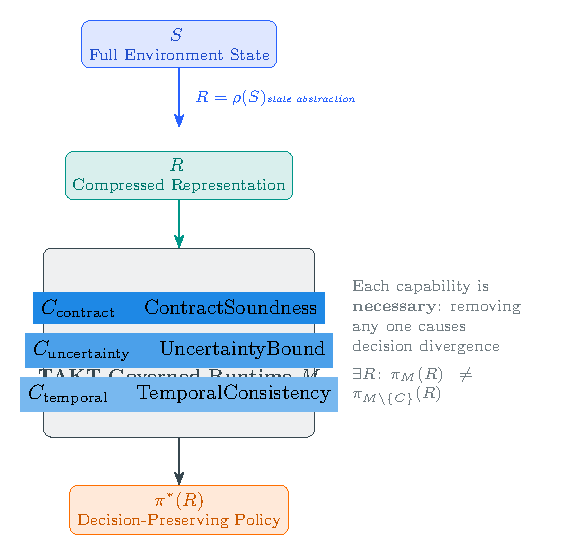
\includegraphics[width=0.85\linewidth]{figures/architecture.pdf}
\caption{Conceptual architecture: TAKT Governed Runtime $M$ enforces decision
preservation $\pi^*(R)$ under state abstraction $\rho(S)$.}
\label{fig:architecture}
\end{figure}

\textbf{Definition (Capability Necessity):} A capability $C \in \mathcal{C}$ is
\emph{locally necessary} for runtime $M$ if removing $C$ alters policy decisions
on at least one representation:
\[
\exists\, R \in \mathcal{R}:\; \pi_M(R) \;\neq\; \pi_{M \setminus \{C\}}(R)
\]

\textbf{Example 1 (Temporal Prefix Necessity):} Consider a runtime where
$C_{\text{temporal}}$ is ablated. Two trajectories $\tau_1 = (r_0, r_1, r_2)$
and $\tau_2 = (r'_0, r'_1, r_2)$ share an identical terminal state $r_2$.
If $\tau_1$ is safe and $\tau_2$ is unsafe, a runtime inspecting only $r_2$
assigns identical actions — causing decision divergence $\pi_M(\tau_1) \neq \pi^*(\tau_1)$.

\section{Machine-Certified Lean 4 Formalization}

The theoretical results establish necessity within the formal model. We implement the proofs in two canonical Lean 4 modules (\texttt{takt-formal}):
\begin{enumerate}
    \item \textbf{\texttt{RuntimeSufficiency.lean}:} Formalizes \texttt{RuntimeCapability}, \texttt{Runtime}, \texttt{removeCapability}, \texttt{PreservesDecision}, \texttt{NecessaryCapability}, \texttt{Sufficient}, \texttt{Irreducible}, \texttt{MinimalRuntime}, proving:
    $$\text{MinimalRuntime}(M, \pi^*) \implies \forall C \in M.\text{capabilities}, \quad \text{NecessaryCapability}(C, M)$$
    \item \textbf{\texttt{RuntimeWitness.lean}:} Defines the 3-layer certification bridge (\texttt{WitnessArtifact}, \texttt{WitnessConsistentWithRuntime} predicate) and proves the elevation theorem:
    $$\text{theorem } \texttt{validWitness\_implies\_necessity} : \text{WitnessConsistentWithRuntime}(M, w) \implies \text{NecessaryCapability}(w.\text{capability}, M)$$
\end{enumerate}

Both Lean 4 modules compile cleanly with zero errors and zero \texttt{sorry}s.

\section{Empirical Validation \& Component Ablation (EXP-004)}

The theoretical theorems prove necessity within the formal model. We validate the
predicted behavior under controlled capability ablations in experiment
\textbf{EXP-004}~\cite{takt_st016_2026}:

\begin{itemize}
    \item \textbf{$C_{\text{contract}}$ Ablation:} Ablating contract verification
    yields $\pi_{\text{full}} = \text{STOP}$ vs.\ $\pi_{\text{reduced}} = \text{EXECUTE}$.

    \item \textbf{$C_{\text{uncertainty}}$ Ablation:} Ablating margin estimation
    at critical decision boundary ($M_D \approx 0$) yields
    $\pi_{\text{full}} = \text{REFINE}$ vs.\ $\pi_{\text{reduced}} = \text{EXECUTE}$.

    \item \textbf{$C_{\text{temporal}}$ Ablation:} Ablating trajectory monitoring
    yields $\pi_{\text{full}} = \text{INTERVENE}$ vs.\ $\pi_{\text{reduced}} = \text{MONITOR}$.
\end{itemize}

Each ablation produces a machine-verifiable \texttt{WitnessArtifact} elevated to
a Lean 4 theorem via the \texttt{validWitness\_implies\_necessity} bridge.

\subsection{Evidence Traceability Matrix}
Table~\ref{tab:evidence} maps each theoretical claim to its primary evidence asset.

\begin{table}[htbp]
\caption{ST-016 Evidence Traceability Matrix}
\label{tab:evidence}
\centering\small
\begin{tabular}{p{3.2cm}p{3.5cm}p{1.4cm}}
\toprule
\textbf{Claim} & \textbf{Primary Evidence} & \textbf{Status} \\
\midrule
Decision Suff.\ ($\Sigma^*$)       & \texttt{StructuralSufficiency} & Verified \\
Kernel Nec.\ ($\mathcal{K}_D$)     & \texttt{RuntimeSufficiency}    & Verified \\
$C_{\text{contract}}$ nec.         & \texttt{contract.ablation}     & Witness  \\
$C_{\text{uncertainty}}$ nec.      & \texttt{uncertainty.ablation}  & Witness  \\
$C_{\text{temporal}}$ nec.         & \texttt{temporal.ablation}     & Witness  \\
Witness bridge                     & \texttt{RuntimeWitness}        & Verified \\
Runtime correctness                & Vitest (283/283)               & Passing  \\
Reproducibility~\cite{takt_st016_2026} & Replication kit           & 6 Runs   \\
\bottomrule
\end{tabular}
\end{table}

\section{Discussion \& Architectural Implications}

The ST-016 results yield three actionable design principles for runtime system
architects. Each principle is grounded in a specific formal or empirical result
from this work.

\begin{enumerate}
    \item \textbf{Safety Contract Decoupling:} Safety verification
    ($C_{\text{contract}}$) cannot be subsumed by statistical policy estimation
    alone. \emph{Grounded in:} EXP-004 ablation of $C_{\text{contract}}$ produced
    EXECUTE on a contract-violating state where the full runtime correctly returned
    STOP. The formal witness artifact was verified consistent with the Lean model.

    \item \textbf{Dynamic Boundary Monitoring:} Operating near ambiguity boundaries
    requires explicit uncertainty estimation ($C_{\text{uncertainty}}$) to prevent
    premature execution. \emph{Grounded in:} EXP-004 ablation of $C_{\text{uncertainty}}$
    at decision margin $M_D \approx 0$ produced EXECUTE where the full runtime
    returned REFINE, with the divergence formally certified via \texttt{RuntimeWitness}.

    \item \textbf{Trajectory History Dependence:} Stateless evaluation fails under
    history-dependent processes, necessitating explicit trajectory prefix tracking
    via $C_{\text{temporal}}$. \emph{Grounded in:} EXP-004 ablation of
    $C_{\text{temporal}}$ produced MONITOR on a history-dependent prefix where
    the full runtime returned INTERVENE (see also Example 1, Section~3).
\end{enumerate}

\section{Scope Boundaries, Non-Claims \& Future Work (ST-017)}
\label{sec:limitations}

\subsection{Non-Claims \& Scope Boundaries}
\begin{enumerate}
    \item \textbf{Model Scope:} ST-016 establishes an algebraic framework and
    witness-based demonstration that $C_{\text{contract}}$, $C_{\text{uncertainty}}$,
    and $C_{\text{temporal}}$ are necessary in formalized finite-instance scenarios.
    It does \emph{not} claim universal necessity for all possible governed runtimes,
    continuous control systems, or runtime models other than the ST-016 formal model.

    \item \textbf{Capability Semantics:} The formal Lean model treats
    $C_{\text{contract}}$, $C_{\text{uncertainty}}$, and $C_{\text{temporal}}$
    as abstract labels. The semantic connection to contract soundness, uncertainty
    bounding, and temporal consistency is established through finite-instance
    examples. General semantic grounding is reserved for future work.

    \item \textbf{Axiom0:} The structural sufficiency module postulates
    $\text{kernel}_D(x,y) \leftrightarrow K_D(x,y)$. This is a modelling
    assumption characterizing the class of decision problems studied, not a
    derived theorem.

    \item \textbf{Witness Bridge Automation:} The formal witness validation schema
    requires manual construction of \texttt{WitnessArtifact} records from
    observed TypeScript traces. No automatic extraction mechanism from runtime
    executions to Lean proofs exists in ST-016.

    \item \textbf{Transportability (ST-017 Boundary):} Transporting certified
    witness artifacts across heterogeneous runtimes ($M_1 \sim M_2$) is reserved
    for \textbf{ST-017}.
\end{enumerate}

\subsection{Open Research Direction: ST016\_Conjecture}
The following claim is \textbf{not proven} in this work and constitutes the
central open research direction for ST-017:

\begin{quote}
\textit{ST016 Conjecture:} For any runtime $M$ with $\mathcal{C} =
\{C_{\text{contract}}, C_{\text{uncertainty}}, C_{\text{temporal}}\}$
and any optimal policy $\pi^*$, if $M$ is decision-preserving then $M$ is
minimal (i.e., no capability can be removed while preserving $\pi^*$).
\end{quote}

Proving this conjecture would require establishing formal semantic axioms for
each capability class and demonstrating irreducibility in a model-independent
way, which is the core research question of ST-017.

\subsection{Conclusion}
ST-016 establishes an algebraic Lean 4 framework for reasoning about minimal
decision-preserving runtime governance, backed by formalized witness scenarios
and an audited replication package. The central open conjecture and semantic
grounding of capability classes provide the foundation for the ST-017 research
line on transportability and generalization.


\bibliographystyle{plain}
\bibliography{bibliography}

\end{document}
